% Chapter Template

\chapter{Model Driven Engineering} % Main chapter title

\label{Chapter2} % Change X to a consecutive number; for referencing this
% chapter elsewhere, use \ref{ChapterX}

\lhead{Chapter 2. \emph{Model Driven Engineering}} % Change X to a consecutive number; this is for the header on each page - perhaps a shortened title

%----------------------------------------------------------------------------------------
%	SECTION 1
%----------------------------------------------------------------------------------------

\section{Introduction}

When a new software is created it has always been a goal to produce high
quality code at the lowest cost. To plan a software development phase from its
initial start to delivering a finished product can seem like an impossible
thing to do. Because a software development cycle rarely goes as initially
planned. Changes do occur, both in delivering high quality code and keeping the
costs down. Traditionally when model driven engineering (MDE) is used, people
think about models, for example activity diagrams and class diagrams from the
popular modeling language, UML. Where models is used to raise the level
of abstraction for the problem specification and describing how a software
should be implemented. For these software development processes models are
indirectly used in the creation of software. This means that models are
primarily used as a reference when implementing an application.

A model is an abstraction of a system, and has its origin from Latin,
\textit{modulus} that means measure or standard. A model can either be used to
represent a system before it is created or to describe some major aspects of a
system or a concept. When we hear the term model, many will think that it
is a miniature that consists of a set of nodes and arrows. But it is important
to consider that a model can also be represented by text. 

If we consider traditionally software development processes, then models are
primarily used in application requirements and use-case diagrams specify what 
the costumer wants. Then developers can specify models to detect important
functionality of the application. The software developer may for example create
flow charts, sequence diagrams, activity diagrams, class diagrams, etc, to
describe how the system should be implemented. A model for system architecture
can also be initialized for developers to handle design choices. Rational
Unified Process\cite{Rational1998} (RUP) is an example of a software
development process that is build around extensive use of models in their
initial planning phase. RUP was initially created by Rational Software
Corporation\cite{IBMRational} in 2006 and was later acquired by International
Business Machines Corporation\cite{IBM}. This is an iterative software
development process and the purpose of RUP is to be an adaptable process
framework where the software project teams decide the elements that are
required for a development cycle. Figure~\ref{fig:RUP} explains the four
different phases, Inception, Elaboration, Construction and Transition, with
different iterations for each phase that RUP provides. The Inception phase and
the Elaboration phase is the two phases where some of the example models above
are created, both under business modeling and requirements. For the Inception
phase of RUP, the idea is to create the software application without writing
any source code. This phase is  concerned with writing text and creating models
that gives the developers a detailed specification on how the program should be
implemented. In the Elaboration phase a prototype might be implemented to show
the customer a possible implementation, but this phase also consist of creating
and modifying an extensive amount text and models that specifies analysis and
design choices. The Elaboration phase focus on designing the architecture for
the software application. The goal for these two phases is to define a solid
foundation of the application before starting with the implementation and
testing. In the Construction phase the developers should know exactly how the
application should be implemented by referring to documents and models created
in earlier phases. RUP is only one example of how a software development
process could be applied to a project. Agile development processes has become
popular the last couple of years, where processes like Scrum\cite{Schwaber2001}
and Extreme Programming\cite{Beck1999} (XP) has been integrated in software
development teams all over the world. Both Scrum and XP thrives to focus more
on the implementation and on delivering high quality code than creating
documents and models. But models will always be a tool for developers, also in
agile development processes, when some aspects of a system needs to be
explained. Because to explain parts of an implementation with a model will help
to make the explanation less complex and more abstract. 

\begin{figure}[H]
	\centering
	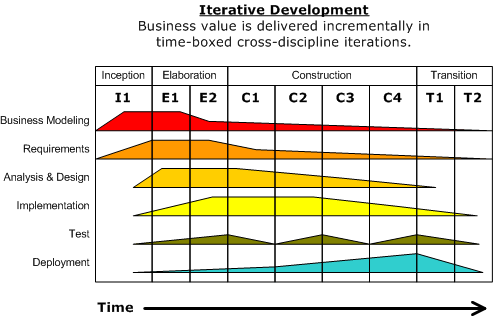
\includegraphics[scale=0.7]{./Figures/RUP.png}
	\caption[Rational Unified Process]
	{Iterative development cycle of Rational Unified Process.}
	\label{fig:RUP}
\end{figure}

Now we have acknowledged some development processes that are commonly used in
the industry for creating software applications. Model Driven Engineering is a
software development methodology which focuses on creating and exploiting
models. And by using these models,  MDE aims at improving productivity and
quality in software development. This is achieved by not only to use models as
documentation, but instead to use models as the major artifact in a software
development cycle. The idea is to use models at different levels of abstraction
and apply model transformations to automate the implementation on these
models.
This will raise the level of abstraction in program and problem specification.
We can divide these models into two main model classes, namely development
models and runtime models\cite{France2007}. Development models is used as an
abstraction above code level. These models could represent software
requirements, work flow, architecture and software implementation. These
development models are most typically used in software development process that
we described above as a supplement in developing an application. Runtime models

\subsection{Model Driven Architecture}

\begin{figure}[H]
	\centering
	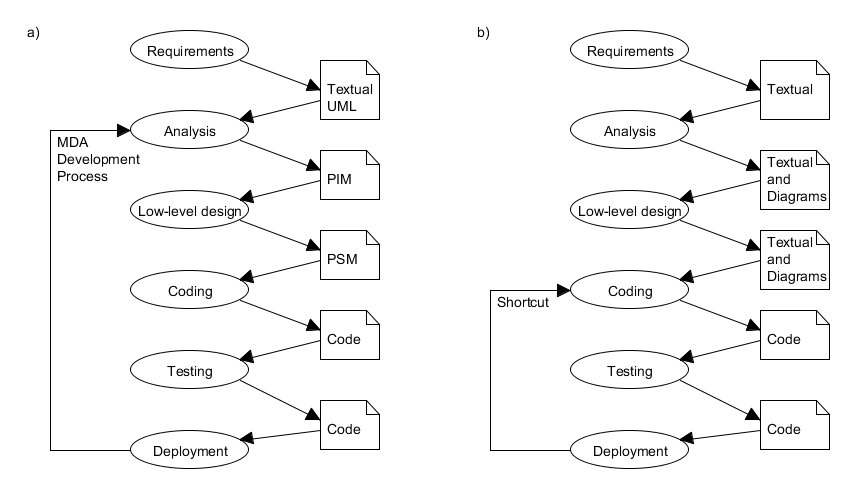
\includegraphics[scale=0.5]{./Figures/MDA.png}
	\caption[Software Development with MDA]
	{a) Model-Driven-Architecture and b) Traditional development process}
	\label{fig:MDA}
\end{figure}



%-----------------------------------
%	SUBSECTION 1
%-----------------------------------
\section{Meta-modeling}

Meta-modeling plays a vital role in model driven engineering (MDE) to describe a
modeling language. A meta-model defines the abstract syntax and provides a
description of a modeling language. Another popular definition for
meta-modeling is that it is a ``model of models". This definition is both
unhelpful and incorrect according to Steve Cook and Stuart Kent in their
paper\cite{Cook2008} published in 2008. They think that a better definition for
a meta-model is that ``it is a model of the concepts expressed by a modeling
language.'' A meta-model is basically a model that is specified by a
meta-modeling language. The exact definition of a meta-model is highly debated
amongst MDE researchers\cite{Rutle_thesis}. When creating instance of these
meta-models we can specify a Domain Specific Modelling Language (DSML) from the
concrete syntax of a meta-model.

\begin{figure}[H]
	\centering
	\includegraphics[scale=0.6]{./Figures/SimpleMeta-model.png}
	\caption[Example of a model and meta-model]
	{A simple example of a model and its meta-model.}
	\label{fig:SimpleMeta-model}
\end{figure}

Figure~\ref{fig:SimpleMeta-model} shows a simple example of a instance model and
its corresponding meta-model. This model has two classes, Student and Course, and
a bidirectional association, take course and has students, that relate
these two classes. The model is specified by a meta-model that consists of two
metaclasses Class and Association and an association between them. Both Student
and Course are an instance of the metaclass Class, while the association
between Student and Course are instance of the metaclass Association. The
modeling language that describes this model corresponds to the Unified Modelling
Language.

The Unified Modeling Language\cite{UML,UML_SPEC} (UML) is a standardized
general-purpose modeling language that was accepted in 2000 by the International
Organization for Standardization (ISO) as an industry standard for modeling
software systems. UML was initially developed by Grady Booch, Ivar Jacobsen and
James Rumbaugh at Rational Software in the 1990s. It was later adopted by the
Object Management Group in 1997 and has since this day been continually
developed by the organisation. 

\subsection{Meta-Object Facility}

The Object Management Group was in need of a architecture to define the
UML. Therefore the Meta-Object Facility has its origin from, that specifies UML.
MOF and is a semi-formal approach to writing meta-models. The Meta-Object
Facility\cite{MOF} (MOF) is an Object Management Group standard for model
driven engineering. According to OMG, this standard provi des a four leveled
architecture.

\begin{figure}[H]
	\centering
	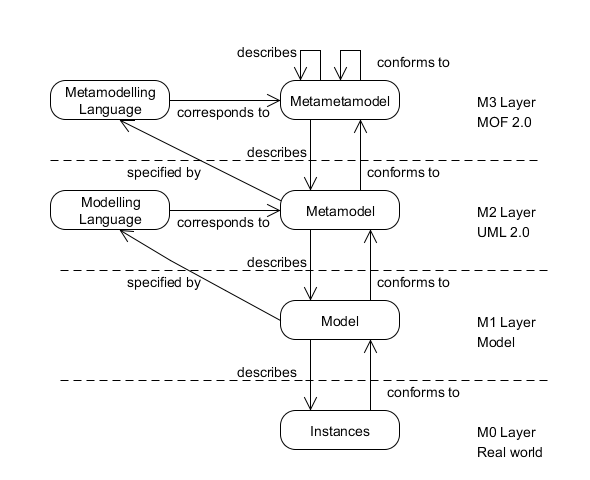
\includegraphics[scale=0.6]{./Figures/MOFLayers.png}
	\caption[Meta Object Facility]
	{Example of Meta Object Facility and its four layers.}
	\label{fig:MOFLayers}
\end{figure}

Figure~\ref{fig:MOFLayers} gives a impression of the four layers that are
available in the Meta-Object Facility. At the top level, M\textsubscript{3}
there is a meta-meta-model called MOF. This meta-meta-model is meant to both
describe it self and conform to itself. This MOF meta-meta-model is then used to
describe meta-models at the M\textsubscript{2} level. The UML meta-model is an
example of such a meta-model. The idea is that these meta-models are specified by
some meta-modeling language. These meta-models at the M\textsubscript{2} layer
describes elements that can be used in the M\textsubscript{1} layer, namely
models. These could be models specified by the modeling language, UML. Finally
at the M\textsubscript{0} we have an instance model of a real world object. 


 

%-----------------------------------
%	SUBSECTION 2
%-----------------------------------



%----------------------------------------------------------------------------------------
%	SECTION 2
%----------------------------------------------------------------------------------------
 
\section{Constraints}

A constraint is a Boolean condition for some modeling element. These modeling
elements can have constraints defined on objects, classes, attributes,
links, associations, etc. A constraint is a restriction on how these
elements should behave. Constraints on elements such as those above can be
expressed with a natural language or by a formal language, such as the
Object Constraint Language\cite{OCL} (OCL). The Object Constraint Language (OCL)
is a declarative programming language for describing constraints that applies to
UML models. Before UML became an adopted standard of the Object Management Group
(OMG), OCL was an extension language to UML. Now OCL can be used with any
Meta-Object Facility (MOF) meta-model, including UML. A software developer
can in combination with UML and OCL specify models. OCL is used as a supplement
to UML, and therefore would refer a to non-existing model element without UML
diagrams\cite{Warmer:2003:OCL:861416}.

The difference between object and classes needs to be specified. A class
is often a meta element for an object. This means that a class could be part of
a model that describes an object element, and therefore an object element is
typed by class element\cite{OO_UML}. Figure~\ref{fig:SimpleMeta-model} describes
the two object elements Student and Course that are an instance of the
meta-element Class.

\begin{figure}[H]
	\centering
	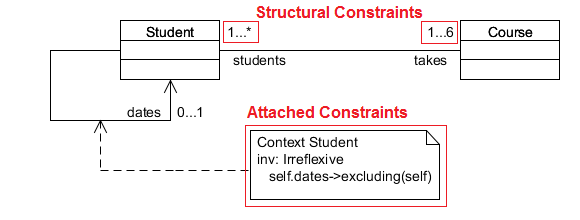
\includegraphics[scale=0.7]{./Figures/Constraints.png}
	\caption[Simple model with constraints]
	{Example of a simple model with attached and structural constraints.}
	\label{fig:Constraints}
\end{figure}

These restrictions on model elements can either be a structural constraint or an
attached constraint. These structural constraints are defined in the structure
of the models. In figure~\ref{fig:Constraints} we have extended the model we
introduced in figure~\ref{fig:SimpleMeta-model} with some  modeling elements. We
have created an association that specifies that a student can date other
students. In this model we can see that the model has three multiplicity
constraints that are part of the models structure. A multiplicity constraint for
an association restricts the number of objects that are related to a given
object. From the association constraint on this model we can see that a student
requires to take at least one course and up to a maximum of six courses. The
models restricts a student to not participate in any courses. The second
structural constraint requires a course to have at least five students for
this course to be part of a semester, and the course can have an arbitrary
maximum number of students participating this course. The association dates,
between two students for this model has an attached constraint, that is
specified in the declarative language OCL. The general form of an attached
constraint has a context, in this case a Student, that specifies what object the
constraint includes. The is a constraint name followed by a Boolean
expression. The attached constraint has a name \textit{``Irreflexive''} followed
by a Boolean OCL expression that explicitly refers to itself. This constraint
specifies that a student is unable to date her or him self. Constraints has a
vital part in model driven engineering to measure the quality and precision of a
model. A model without constraints does not work in practice. In
\textit{The Object Constraint Language: Getting Your Models Ready for
MDA}\cite{Warmer:2003:OCL:861416}, Jos Warmer and Anneke Kleppe states that a
model without constraints would be severely underspecified. Constraints
expressions written in OCL are unambiguous and results in a more precise and
detailed model. If we where to remove both the structural and attached
constraints from figure~\ref{fig:Constraints} then the model is less
informative. There is no understanding on how the objects are related to
one another. 

\section{Workbenches}

\subsection{Eclipse Platform}

\begin{figure}[H]
	\centering
	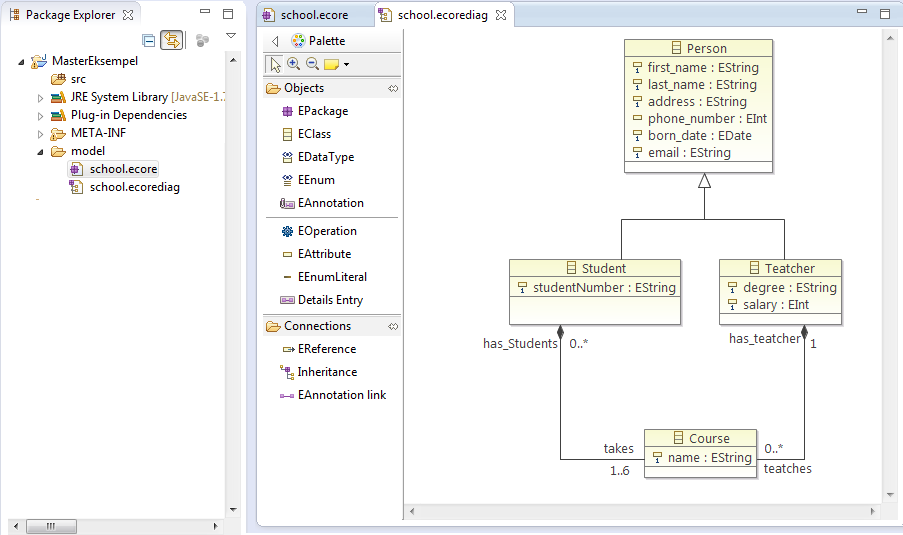
\includegraphics[scale=0.6]{./Figures/EMF_Diagram_Picture.png}
	\caption[Ecore model represented by Ecore Tools]
	{A graphical representation of an Ecore model.}
	\label{fig:EMF_Diagram}
\end{figure}

\begin{figure}[H]
	\centering
	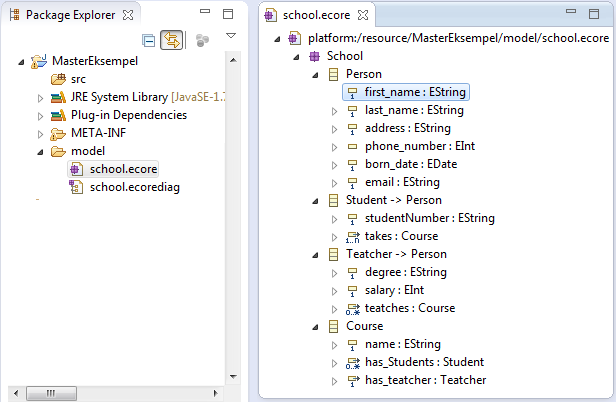
\includegraphics[scale=0.8]{./Figures/EMF_Ecore_Picture.png}
	\caption[Tree based representation of an Ecore model]
	{Tree based representation of an Ecore model.}
	\label{fig:EMF_Ecore}
\end{figure}

\begin{figure}[H]
	\centering
	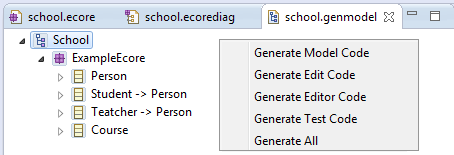
\includegraphics[scale=0.7]{./Figures/EMF_GenModel.png}
	\caption[Representation of an EMF Generator model]
	{Representation of a generated EMF Generator model.}
	\label{fig:EMF_Ecore}
\end{figure}

\subsubsection{EMF}

In EMF we can create data models based on the Essential MOF (EMOF) and specify
domain specific languages. The Henshin meta-model is created as an EMF
meta-model and uses the Ecore meta-model for typing purposes.

EMF will generate interfaces and factory

With EMF you make your domain model explicit which helps to provide clear
visibility of the model. EMF also provides change notification functionality to
the model in case of model changes. EMF will generate interfaces and factory to
create your objects; therefore it helps you to keep your application clean from
the individual implementaiton classes.

\section{DPF}

Diagram Predicate Framework\cite{Rutle_thesis,Rossini_thesis,Lamo2013} (DPF) is
an ongoing research project that was first initiated by Bergen University
Collage and the University of Bergen in Norway 2006. With features likes
meta-modeling, model transformation and model management, DPF aims at
formalising concepts of model-driven engineering. DPF is based on category
theory and graph transformations and is an extension of the Generalised
Sketches\cite{Diskin2003} formalism that was initially developed by Zinovy
Diskin.

In October 2002 Dominique Duval published a paper where he specified that a
specification can be considered as a directed graph with additional structure
in the same way that a theory can be considered as a category with additional
structures\cite{Duval2003}. Generalised Sketches by Zinovy Diskin utilize the
concept of sketches. A sketch, first introduced by Ehresman in 1966, is a
directed graph that provides additional properties, such as colimit, limit and
constraints. DPF utilize this concept through an diagrammatic approach to
meta-modeling and to facilitate the concepts of MDE. The framework provides the
possibility to define an unlimited layers of meta-modeling. In DPF models are
represented as specifications. 

\begin{itemize}
  
\item A \emph{specification $\spec{S}$} = (S,
C\textsuperscript{$\spec{S}$}:$\Sigma$) consist of an underlying graph S and a
set of atomic constraints C\textsuperscript{$\spec{S}$}. 

\item Atomic constraints are specified by predicates, that is a Boolean value
function, from a predefined signature $\Sigma$.

\item A signature $\Sigma$ = ($\Pi$ \hspace{1 mm}, \hspace{1 mm}$\alpha$)
consist of a collection of predicates. 
  
\end{itemize}

A \emph{specification $\spec{S}$} has an underlying graph S that contains
modeling elements that defines the model structure of the specification. These
modeling elements are always represented as a node and an arrow. However these
nodes and arrows could be specified through several underlying layers of
meta-models or specifications. The \emph{specification $\spec{S}$} also consist
of a set of constraints, these constraints will restrict the model structure of
a new instance model of this specification. Figure~\ref{fig:DPF_Spec} presents a
specification $\spec{S}$\textsubscript{2}, that is defined by an underlying
specification $\spec{S}$\textsubscript{3} and describes a modeling language for
some $\spec{S}$\textsubscript{1} specification. This specification includes two
nodes Condition and Activity, two arrows ChoiceOut and Message and  two sets of
atomic constraints. The first constraint defines that a Condition element has
to be connected to exactly one Activity element for this structure. The second
constraints specifies for this graph structure that an Activity element cannot
be associated with it self. These constraints examples are specified as a
collection of predicates from a predefined signature $\Sigma$. The table in
figure~\ref{fig:DPF_Spec} represent some of the predicates from this
collection. A predicate is represented by an unique symbol $\Pi$, a shape graph
$\alpha$, a proposed visualisation and a semantic interpretation

\begin{figure}[H]
	\centering
	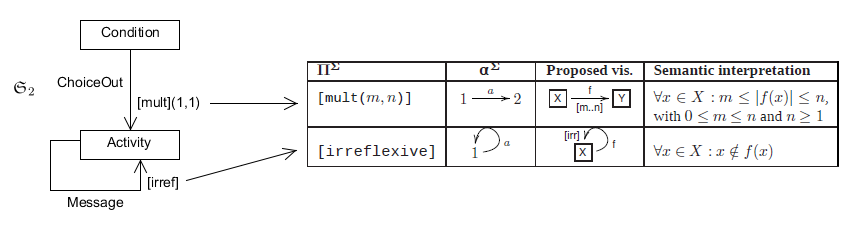
\includegraphics[scale=0.7]{./Figures/DPF_spec_constraints.png}
	\caption[A specification and some predefined diagrammatic predicate attached]
	{A specification $\spec{S}$\textsubscript{2} with some attached predicates.}
	\label{fig:DPF_Spec}
\end{figure}

An instance specification $\spec{S}$\textsubscript{n} that is initialised from
a specification $\spec{S}$\textsubscript{n+1} defines a graph homomorphism
between two underlying graphs. There is a graph homomorphism,
T$\longrightarrow$S, between the underlying graph T of
$\spec{S}$\textsubscript{n} and the underlying graph S of
$\spec{S}$\textsubscript{n+1}\cite{Lamo2013}. This graph homomorphism
T$\longrightarrow$S must satisfy the set of atomic constraints,
C\textsuperscript{$\spec{S}$} from the specification
$\spec{S}$\textsubscript{n+1}. The nodes and arrows that are defined in the
underlying graph S from a specification $\spec{S}$\textsubscript{n+1} describes
the modeling elements that a specification $\spec{S}$\textsubscript{n} can use
to create a graph structure.

\cite{Brambilla:MDSE}

\begin{figure}[H]
	\centering
	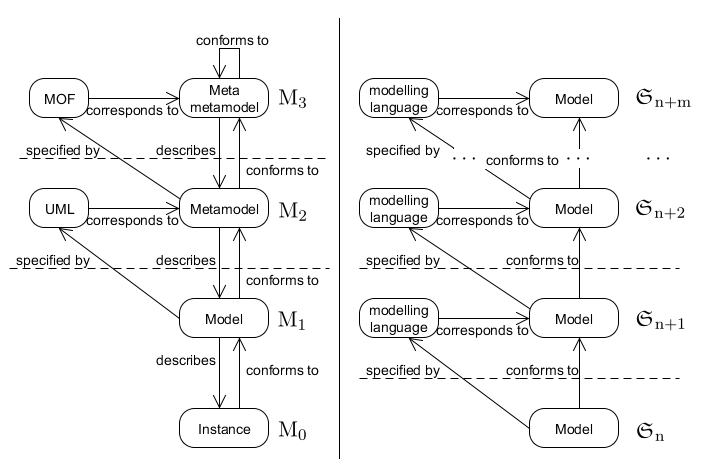
\includegraphics[scale=0.7]{./Figures/MOF_vs_DPF}
	\caption[OMG's layers of meta-modeling and multilayer modeling]
	{OMG's layers of meta-modeling and an arbitrary layer of meta-modeling.}
	\label{fig:MOF_vs_DPF}
\end{figure}



 
\section{DPF Editor}

 
\begin{table}[ht]
\renewcommand*\arraystretch{1.5}
\centering
\begin{tabular}{| c | c | c | c | c | c |}
\hline
Tool & Layers & Dia.   & Const.   & Platform & GUI\\
	 & 		  & Const. & Language &          & \\
\hline
EMF/GMF & 2 & & OCL, EVL, & Java VM & $\surd$ \\
		&  	& & Java      &         & \\
\hline
VMTS    & $\infty$ & & OCL & Windows & $\surd$ \\
\hline
AToM\textsuperscript{3} & 2 & & OCL, Python & Python, Tk/tcl & $\surd$ \\
\hline
GME  & 2 & & OCL & Windows & $\surd$ \\
\hline
metaDepth & $\infty$ & & EVL & Java VM & \\
\hline
DPF & $\infty$ & $\surd$ & Predefined & Java VM & $\surd$ \\
	& 		   &         & validator  &         & \\
\hline

\end{tabular}
\caption{Comparing model transformation tools.}
\end{table} 